\section{Auswertung}

\subsection{Nulleffekt}
Die gemessen Impulse ohne Präparat in einem Intervall von $\Delta t = 300\si{s}$ sind in Tabelle \ref{tab:ogemessdaten4} angegeben.
%\begin{equation*}
%N_U= \{ 129, 143, 144, 136, 139, 126, 158 \}
%\end{equation*}
Da es sich um Zählraten handelt werden zunächst alle Fehler der Messwerte aus Tabelle \ref{tab:ogemessdaten4} mit einer Poissonverteilung bestimmt.
\begin{equation}
\label{eqn:poisson}
\increment N_{i} = \sqrt{N_{i}}
\end{equation}
Die Ergebnisse stehen in der folgenden Tabelle \ref{tab:fehleraufn}.
\begin{table}
\centering
\caption{Statistische Fehler auf die Untergrundraten.}
\label{tab:fehleraufn}
\begin{tabular}{c c}
    \toprule
    Untergrundrate $N_{U}$[$\text{Imp}$/$300\si{\second}$] & Fehler $\increment N_{U}$[$\text{Imp}$/$300\si{\second}$]\\
    \midrule
    129{,}00 & 11{,}36\\
    143{,}00 & 11{,}96\\
    144{,}00 & 12{,}00\\
    136{,}00 & 11{,}66\\
    139{,}00 & 11{,}79\\
    126{,}00 & 11{,}22\\ 
    158{,}00 & 12{,}57\\
    \bottomrule
\end{tabular}
\end{table}
Anschließend können diese Werte gemittelt werden, dabei gilt
\begin{equation}
\overline{N_{U}} = \frac{1}{n} \sum_{i=1}^n N_{U_{i}}
\end{equation}
sowie mit einer Gaußschen Fehlerfortpflanzung die Fehler auf diesen Mitteltwert.
\begin{equation}
\increment \overline{N_{U}} = \sqrt{\sum_{i=0}^{n} \left( \frac{\text{d}\overline{N_{U}}}{\text{d}N_{U_{i}}}\right)^{2} (\increment N_{U_{i}})^{2}}
\end{equation}
Daraus ergibt sich eine Untergrundrate mit einem Fehler welche in den nachfolgenden Rechnungen der Auswertung subtrahiert werden können.
\begin{equation}
\overline{N_{U}} = \SI{139.29(446)}{{\text{Imp}}\per{300}\second}
\end{equation}
Für die Auswertung werden diese Angaben für jeweils $\si{{\text{Imp\per}{15}}\second}$ und $\si{{\text{Imp\per}{30}}\second}$ gebraucht, dazu werden die Messwerte aus Tabelle \ref{tab:ogemessdaten4} zunächst 
auf die jeweilige Einheit gebracht und dann die analoge Rechnung durchgeführt. Es ergibt sich
\begin{align}
\overline{N_{U_{15}}} &= \SI{6.96(424)}{{\text{Imp}\per{15}\second}} \\                %schöner machen
\overline{N_{U_{30}}} &= \SI{13.93(141)}{{\text{Imp}\per{30}\second}}
\end{align}

\subsection{Bestimmung der Halbwertszeit von Vanadium}

Zunächst müssen die Messwerte in Tabelle \ref{tab:Vanadium} wieder durch eine Poissonverteilung bestimmt werden.
Hierbei gilt wie zuvor die Gleichung \ref{eqn:poisson}. Die Fehler auf die Messwerte sind bereits in der 
Tabelle \ref{tab:Vanadium} mit eingetragen.
\\
\newline
Die zuvor bestimmte Untergrundrate $N_{U}$ in $\si{{\text{Imp\per}{30}}\second}$ muss nun von der fehlerbehafteten Zählrate
$N_{\text{gem}}$ abgezogen werden. Also gilt,
\begin{equation}
N_{\text{Vanadium}} = N_{\text{gem}} - \overline{N_{U_{30}}}
\end{equation}
wobei wieder eine Gaußsche Fehlerfortpflanzung nötig wird. Der Fehler auf $N_{\text{Vanadium}}$ berechnet sich wie folgt.
\begin{equation}
\increment N_{{\text{Vanadium}_{i}}} = \sqrt{N_{{\text{gem}_{i}}} + (\overline{\increment N_{U_{30}}})^{2} }
\end{equation}
Die ermittelten Werte lassen sich nun in eine halblogarithmische Darstellung einzeichnen wobei eine lineare Ausgleichsgerade
von der Form
\begin{equation}
y = a \cdot x + b
\end{equation}
mit einem linearen Fit bestimmt werden kann. Die Parameter ergeben sich zu
\begin{align}
a &= \SI{-3.17(16)}{\per\milli\second} \\
b &= \SI{5.187(128)}{}
\end{align}
Die Zählwerte $N_{\text{Vanadium}}$ mit Ausgleichsgerade sind in Diagramm \ref{fig:plot2} halblogarithmisch dargestellt, wobei in dieser Darstellung die Gerade wieder exponentiell angehoben werden muss damit sie linear erscheint, dies lässt sich
an der Gleichung \eqref{eqn:g2} erkennen.
Wenn die Zählraten logarithmiert werden wie in Gleichung \eqref{eqn:brrr} entsteht ein Bild wie in Diagramm \ref{fig:plot1}.
\\
\newline
An der Gleichung \eqref{eqn:g2} lässt sich nun erkennen, dass der Parameter $a = -\lambda$ entspricht. Somit ergibt sich für die 
Zerfallskonstante $\lambda$.
\begin{equation}
\lambda = \SI{3.17(16)}{\per\milli\second} 
\end{equation}
Daraus folgt die Halbwertszeit aus dem Zusammenhang \eqref{eqn:187} durch Einsetzen von $\lambda$.
\begin{equation}
T_{\text{Vanadium}} = \frac{\text{ln}2}{\lambda} = \SI{218.66(1104)}{\second} \quad  \widehat{=} \quad \SI{3.64(18)}{\minute}
\end{equation}
Wobei sich der Fehler aus der folgenden Gaußschen Fehlerfortpflanzung ergibt.
\begin{equation}
\increment T_{\text{Vanadium}} = \frac{\text{ln}(2)}{\lambda^{2}} \cdot (\increment \lambda)
\end{equation}
%Der Fehler auf den Mitteltwert lässt sich nun wie folgt angeben.
%\begin{align*}
%\increment{\overline{N}} &= \sqrt{\frac{1}{n(n-1)} \sum_{k=1}^n (N_{i} - \overline{N})^2} \\[2.5pt]
%\increment{\overline{N}} &= \SI{4.02}{{\text{Imp}}\per{300}\second}
%\end{align*}
%Da der Wert $\overline{N}$
%\begin{equation}
%\overline{N} = \SI{139.29(402)}{{\text{Imp}}\per{300}\second}
%\end{equation}
%eine Zählrate ist, unterliegt sie einer Poissonverteilung.
%\begin{align}
%\label{eqn:mittel}
%\Delta N &= \sqrt{N}
%\intertext{Diesen gilt es wiederum über die Anzahl der Messungen zu mitteln}
% \overline{\Delta N} &= \frac{1}{n} \sum_{i=1}^n \Delta N_i% BAR MUSS GRÖ?ER
%\intertext{mit entsprechende werten (siehe Anhang) ergibt sich als Mitteltwert der Poisson Verteilung und somit als finalen Wert des Nulleffekts} % idk obd as schön ist, bzw ob das geht
%\overline{\Delta N} & = \si{139}{\pm4}
%\end{align}
%Die Fehler der gemessenen Werte des Nulleffekts werden jeweils durch eine Poisson Verteilung herausgefunden.
%Da es eine Vielzahl an Messungen gibt, werden die resultierenden Fehler anschließend gemittelt.
%Dabei sieht der Fehler auf den Mittelwert $\overline{N}$ wie folgt aus
%\begin{align}
%\increment{\overline{N}} &= \sqrt{\overline{N}}\\
%\label{}
%\end{align}
%Das Mittel des Nulleffekts auf einem Intervall von $\Delta t = 300\si{s}$ ist nun also bekannt. Um den Effekt auf die kommenden Aufgaben anzupassen 
%wird $\overline{\Delta N}$ mit einem Dreisatz, den Fehler natürlich miteinbeziehend, angepasst. 
%\begin{align}
%\overline{\Delta N_{30}} &= 13.9\pm 0.4 [\frac{Imp}{30\si{s}}] \\                %schöner machen
%\overline{\Delta N_{15}} &= 6.96\pm 0.22 [\frac{Imp}{30\si{s}}]
%\end{align}
%\\
%\paragraph{Mittelung der Messwerte von Vanadium} \mbox{} \\
%Analog zu \eqref{eqn:mittel} lässt sich durch die Poisson Verteilung der Fehler auf  die Werte bestimmen. Die genauen Ergebnisse befinden sich im Anhang.

%\begin{figure}
%  \centering
%  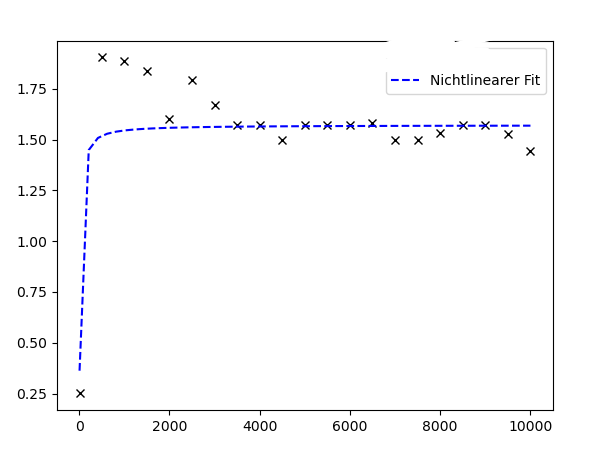
\includegraphics[width=0.8\textwidth]{build/plot1.pdf}
%  \caption{$t-N$ Diagramm.}
%  \label{fig:tndiagramm}
%\end{figure}

\begin{figure}[h]
  \centering
  \includegraphics[width=\textwidth]{build/plot2.pdf}
  \caption{Messwerte und Ausgleichsgerade in halblogarithmischer Darstellung}
  \label{fig:plot2}
\end{figure}


\begin{figure}[h]
  \centering
  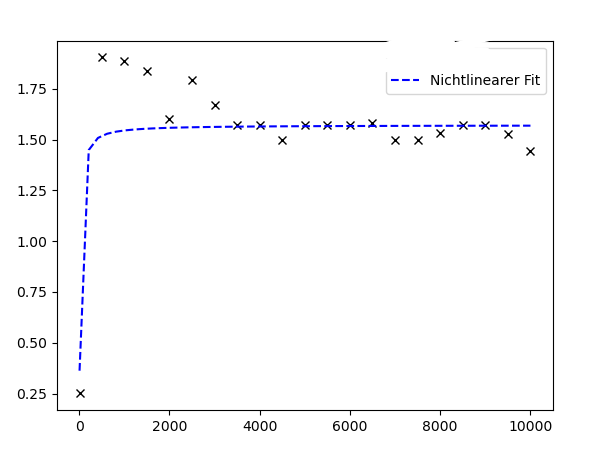
\includegraphics[width=\textwidth]{build/plot1.pdf}
  \caption{Messwerte und lineare Ausgleichsgerade.}
  \label{fig:plot1}
\end{figure}




